\chapter{Introduction}

%\section{Context}

\begin{itemize}
	% context 
	% complex systems
	
	\item Nowadays devices are becoming more complex. They embed several subsystems with different characteristics that communicate and interact in many ways. For example, current cars can integrate an adaptive control cruise system, GPS tracking, fuel control system and soon on. Furthermore, these subsystems are widely coupled. For instance, the adaptive cruise system controls the way to get home depending on the GPS tacking, also, the fuel control system regulates the speed of the car depending on the level of fuel.
	
	% designing of complex systems
	\item This makes the designing of these systems very complex. A designer has to dealt with the heterogeneity of each subsystem but also with the interaction between them. To reduce the complexity of such a development, the designing is split into different domains, \eg mechanical, electronic, software. Therefore, the development of such complex system is talcked by different domains experts.
	
	% Multiple DSMLs --> heterogenenous
	\item In this context, Model Driven Engineering (MDE) has addressed the problem of the development of application for complex systems by proposing Domain Specific Modeling Languages (DSMLs). Each domain expert relies on a DSMLs to better describe its domain. Each DSMLs has its own expressiveness and properties. As a result of such development, several models conforming to different DSMLs are developed and the specification of the overall system becomes \emph{heterogeneous}.
% problem
	\item At some point of development, these models have to be integrated to understand the system and its emerging behavior globally. It is necessary to specify how models and languages are related to each other, in both a structural and a behavioral way. The GEMOC initiative has addressed this problem by proposing to coordinate and disseminate the research results regarding the support of the coordinated use of various modeling languages that will lead to the concept of globalization of modeling languages, that is, the use of multiple modeling languages to support coordinated development of diverse aspects of a system. This thesis is part of GEMOC initiative. We focus on the coordination~\cite{coordsignibib} of behavioral models/languages to provide simulation and/or verification capabilities for the whole system specification. 
	
	
% partial solution
	\item Coordination Languages~\cite{coordsignibib} and Architecture Description Languages (ADLs)~\cite{frameadlsbib} provide dedicated languages to specify the coordination between particular behavioral models. This is usually done by system designers that apply some coordination patterns according to their own skills and know-how. To automate such a task, coordination frameworks~\cite{ptoleframebib,modhelxbib} have identified such a pattern and they have encoded it inside a tool, \eg Ptolemy~\cite{ptoleframebib}, Modhel'X~\cite{modhelxbib}. However, the semantics of the coordination is hidden thus limiting reasoning. Furthermore, they rely on a general purpose language to express the coordination thus limiting verification and validation of the coordinated system. Since the coordination pattern is encoded, they prevent any tunning of the pattern.   
	
% contribution
\item In this thesis, we deal with the coordination of heterogeneous behavioral models by leveraging on the system designer's skills. We propose a dedicated language named \bcool (standing as Behavioral Coordination Operator Language) that allows for capturing coordination patterns for a given set of DSMLs. These patterns are captured between languages, and then used to derive a coordination model automatically for models conforming to the targeted DSMLs. The coordination at the language level relies on a so-called \emph{language behavioral interface}. This interface exposes an abstraction of the language behavioral semantics in terms of Events. \bcool helps understand and reason about the relationships between different languages used in the design of a system.  

\item In \bcool, an integrator can define operators to specify how events from different language behavioral interface interact. These operators are defined at language level but they are applied between models to coordinate their behavior. This results in a model of coordination in \ccsl, a declarative language that describes causal and temporal relationships between events. By relying on \ccsl, we provide verification and validation of the coordinated system.    

% outline	 		
\item The content of this thesis is organized as follows. 

\item Chapter~\ref{ch:background} presents the background about the integration of structural and behavioral models. We categorize the background into approaches that compose models and approaches that coordinate models. In particular, we focus on approaches that have captured coordination pattern between languages in order to automate the coordination between models.   

\item In Chapter~\ref{ch:framework}, we present a framework to characterize coordination pattern approaches. We use this framework to compare different approaches. From this study, we propose the requirements for a language to capture coordination patterns, \ie \bcool.  

\item In Chapter~\ref{ch:bcool}, we elaborate on our approach by presenting \bcool. We introduce a running example that we use all through the chapter to illustrate the syntax and semantics of \bcool. Then, we show the current implementation of \bcool in the GEMOC studio by executing and validating the heterogeneous model of a coffee machine. 

\item Chapter~\ref{ch:examples} validates our approach by presenting the different facets of the developing of a complex heterogeneous system by developing a set of operators between TFSM and Activity. 

%\item Section~\ref{sec:coord-lang} presents the main issues in the coordination of behavioral models, and shows how they can be tackled by explicitly capturing coordination patterns at the language level. Section~\ref{sec:interfaceandexample} defines the notion of language behavioral interface by using an example language named Timed Finite State Machine (TFSM). This language is used later in Section~\ref{sec:BCOol} to illustrate \bcool. In Section~\ref{sec:caseStudies}, we validate the approach by using \bcool to capture three coordination patterns between two languages: TFSM and fUML Activities. Section~\ref{sec:related} gives an overview and comparison to related work. Section~\ref{sec:conclu} concludes with a brief summary and a discussion of ongoing and future actions.
	
%\item Finally, we provide the conclusion of this work, highlighting its main contributions and we give some future perspectives in Chapter 7.
	
\end{itemize}

%\begin{landscape}
%\begin{figure}
%	\begin{center}
%		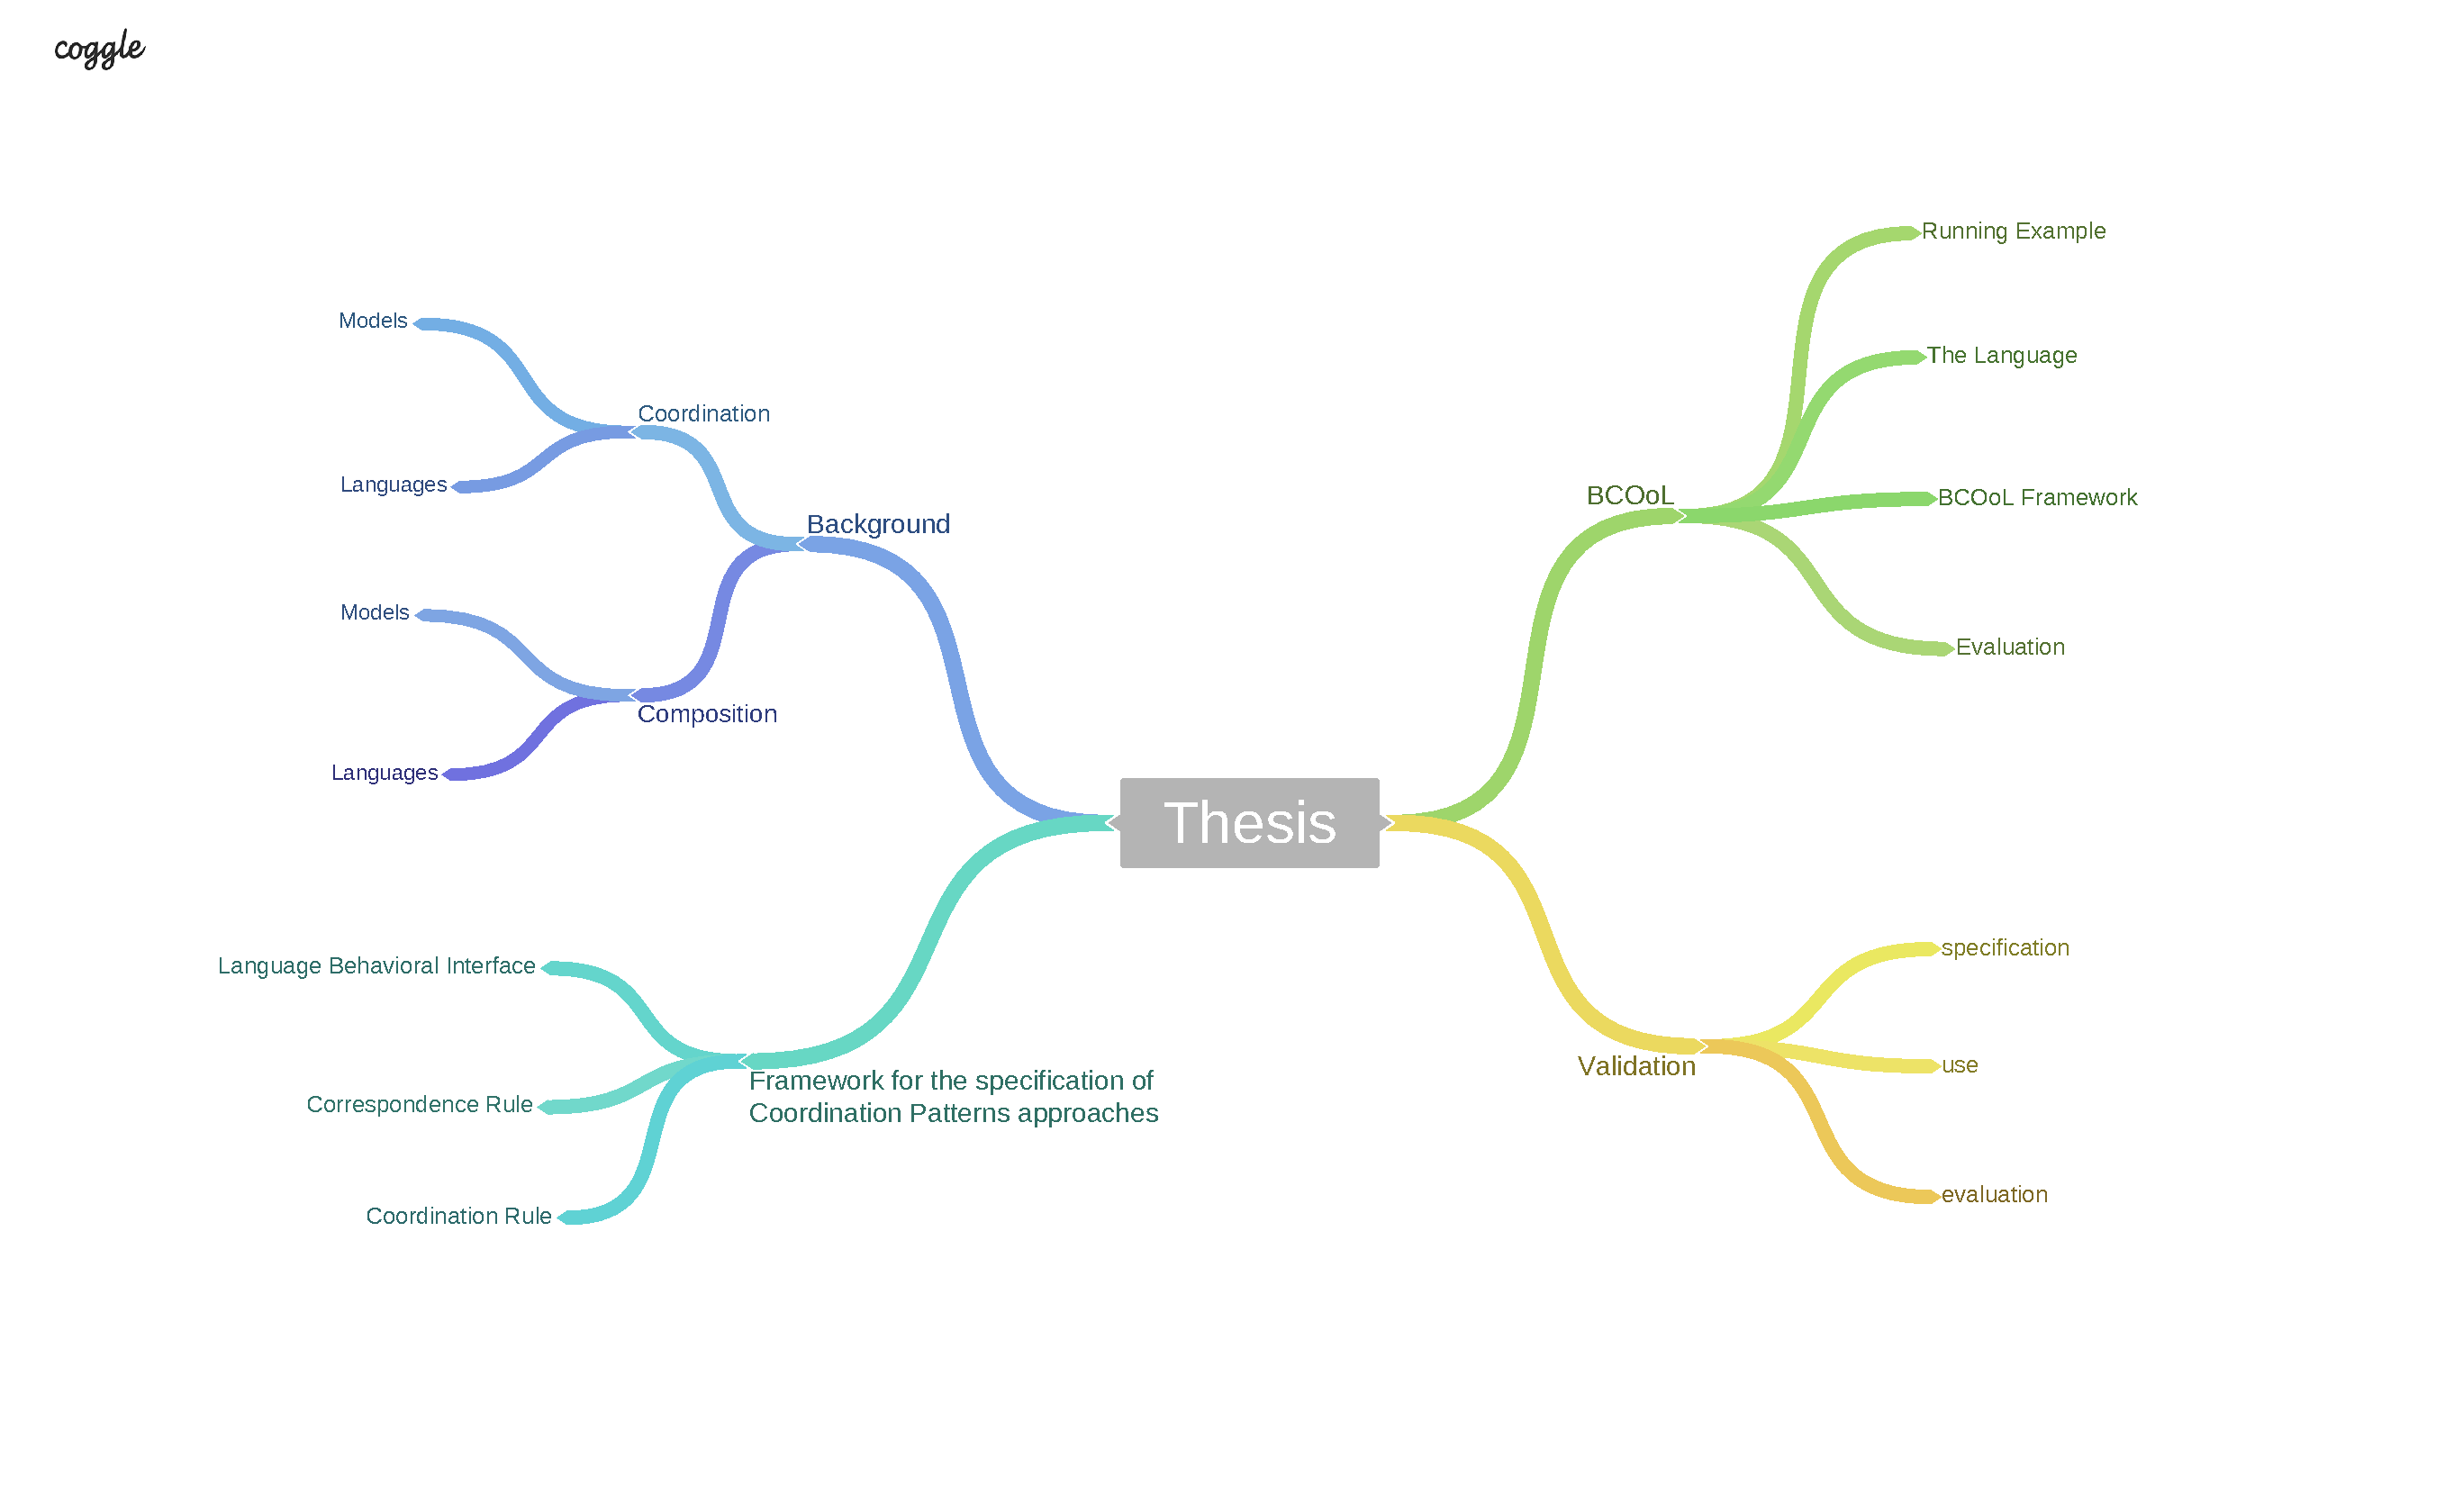
\includegraphics[width=1\textwidth]{Thesisoutline.pdf}
%		\label{fig:thesis outline}
%	\end{center}
%\end{figure}
%\end{landscape}

%\section{Problem}

%\section{Contributions}

%Contributions here.

%\section{Publications}

%Publications here.